\subsection{Model Validation}

Figure~\ref{fig:timely_model_validation} compares the TIMELY fluid model with
the packet-level simulations using the NS3 simulator~\cite{ns3}. The parameters
values are shown in Table~\ref{tab:timely_model_validation}, and are based on
guidance provided in\cite{timely}.  We model a simple topology, in which N
senders, connected to a switch, send to a single receiver, also connected to
that switch. We see the fluid model and the simulator are in good agreement,
barring some time shift in queue behavior.

The ns3 simulations shown in Figure~\ref{fig:timely_model_validation} differ
from the TIMELY implementation in one important aspect. The simulator controls
rate by adjusting delay between individual packets. However, doing so in the
real world would require hardware rate limiters. As an engineering compromised
(i.e. to avoid the dependence on hardware rate limiters), the TIMELY
implementation controls rate by adjusting delay between successive transmissions
of chunks that can be as large as 64KB. Each chunk is sent out at line rate.  In
Figure~\ref{fig:timely_sim_bursty} we simulate this bursty behavior for two
flows, for chunk sizes of 16KB and 64KB.

These results clearly demonstrate that TIMELY behaves poorly with larger chunk
sizes. The initial chunks sent by the two senders arrive at the switch
near-simultaneously (i.e. ``incast''), and both flows receive a very large RTT
sample. This causes TIMELY to reduce its rate drastically (line 8 in the TIMELY
algorithm). Since the subsequent rate increase occurs in small steps ($\delta =
10Mbps$, see line 6.), it takes a long time for the flow rates to climb back to
their fair share.

Needless to say, the equations in Figure~\ref{fig:timely_model} model the
``ideal'' TIMELY behavior (infinitely small chunk size) -- and the actual
behavior will approach the ideal one as chunk size is reduced (see results for
16KB chunk size).

\begin{table}[t]
\small
\center
\begin{tabular}{c|c}
Parameter & Value \\ \hline
C & 10Gbps \\ 
$T_{low}$ & 50 $\mu$s \\ 
$T_{high}$ & 500 $\mu$s \\
$D_{minRTT}$ & 20 $\mu$s \\
$\beta$ & 0.8 \\
$\alpha$ & 0.875 \\
$\delta$ & 10Mbps
\end{tabular}
\caption{TIMELY parameter values for model validation}
\label{tab:timely_model_validation}
\end{table}

\begin{figure}[t]
\center
\subfigure[N=2] { 
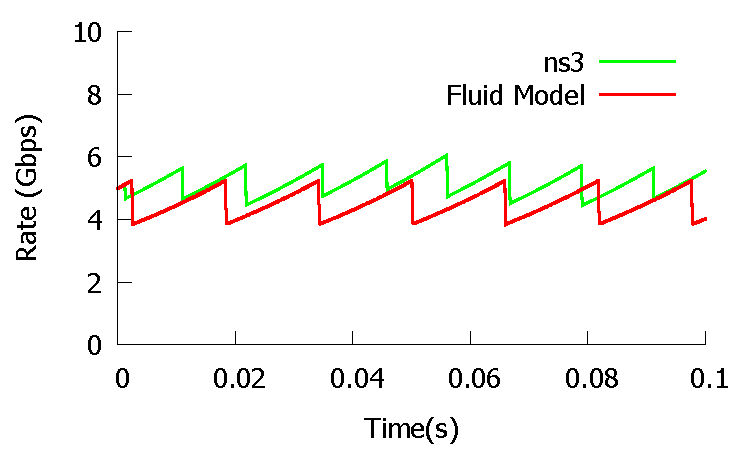
\includegraphics[width=0.45\columnwidth]{figures/timely_validation_2_rate.pdf}
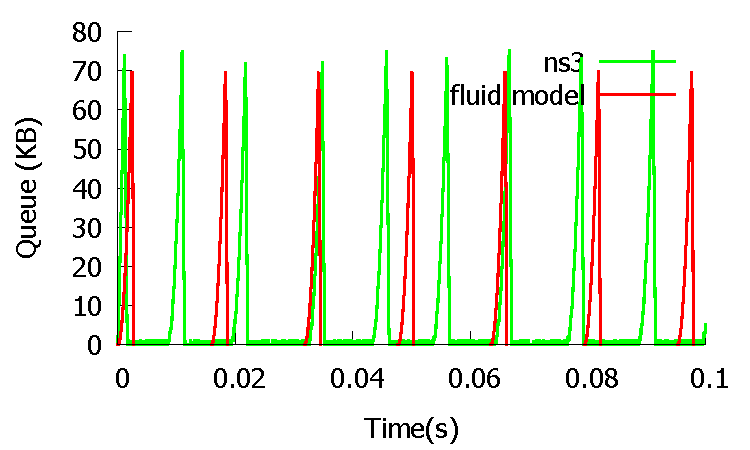
\includegraphics[width=0.45\columnwidth]{figures/timely_validation_2_q.pdf}
}
\subfigure[N=10] { 
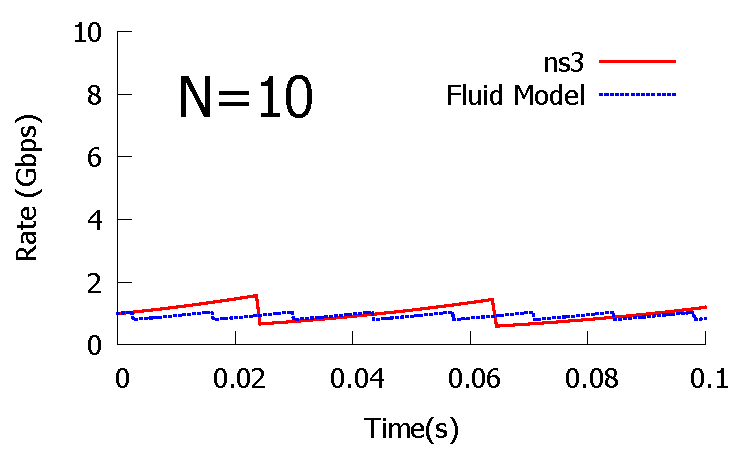
\includegraphics[width=0.45\columnwidth]{figures/timely_validation_10_rate.pdf}
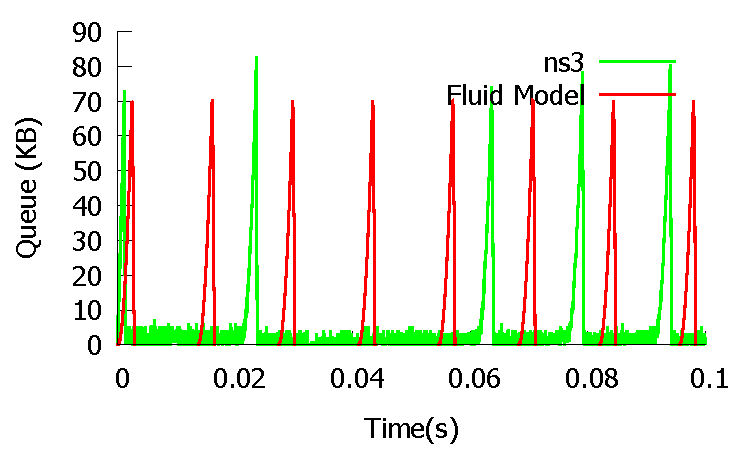
\includegraphics[width=0.45\columnwidth]{figures/timely_validation_10_q.pdf}
}
\subfigure[N=20] { 
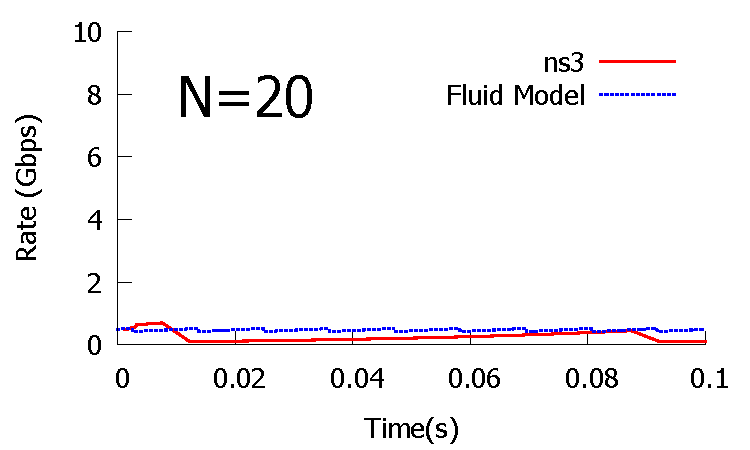
\includegraphics[width=0.45\columnwidth]{figures/timely_validation_20_rate.pdf}
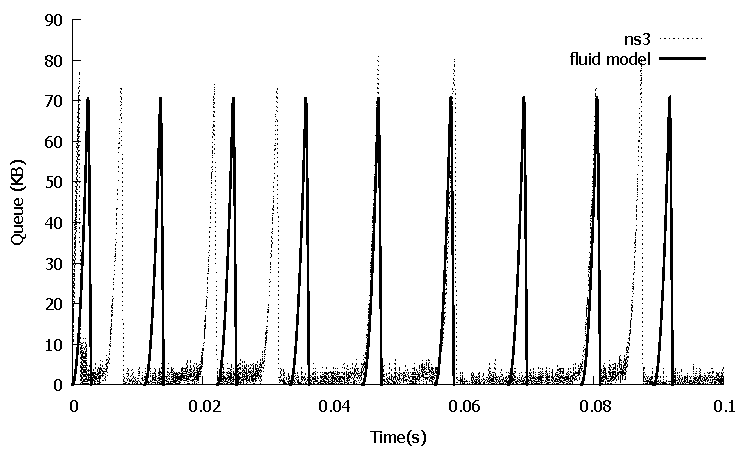
\includegraphics[width=0.45\columnwidth]{figures/timely_validation_20_q.pdf}
}
\caption{Comparison of TIMELY fluid model and simulations}
\label{fig:timely_model_validation}
\end{figure}

\begin{figure}[t]
\center
\subfigure[N=2, 16KB chunk] { 
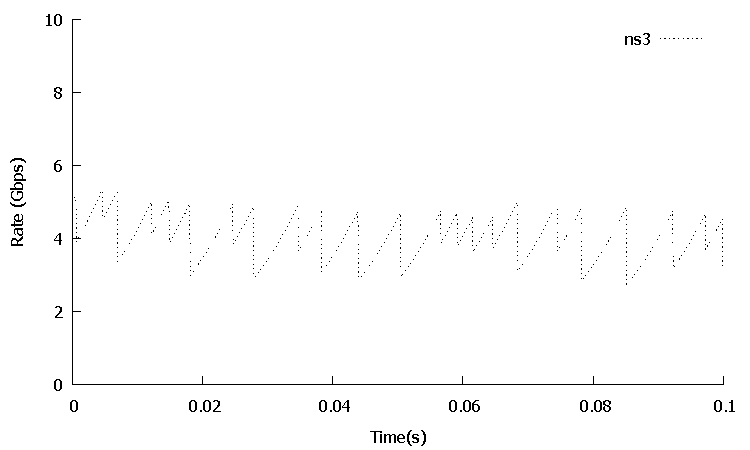
\includegraphics[width=0.4\columnwidth]{figures/timely_bursty_16_rate.pdf}
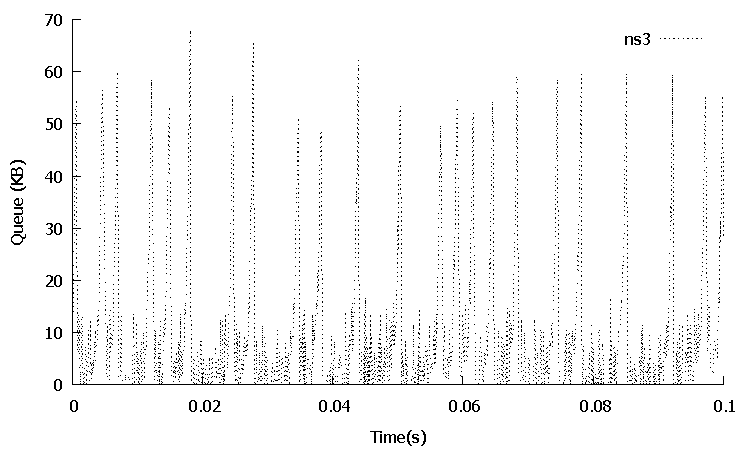
\includegraphics[width=0.4\columnwidth]{figures/timely_bursty_16_q.pdf}
}
\subfigure[N=2, 64KB chunk] { 
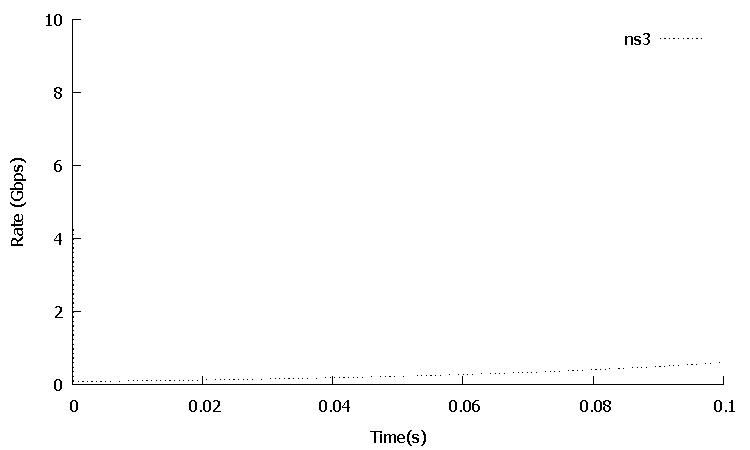
\includegraphics[width=0.4\columnwidth]{figures/timely_bursty_64_rate.pdf}
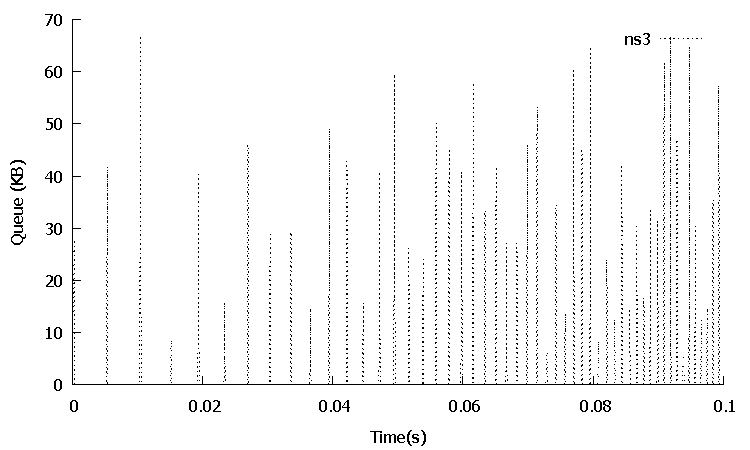
\includegraphics[width=0.4\columnwidth]{figures/timely_bursty_64_q.pdf}
}
\caption{TIMELY with chunk-based rate limiting}
\label{fig:timely_sim_bursty}
\end{figure}


